


\tikzset{every picture/.style={line width=0.75pt}} %set default line width to 0.75pt        

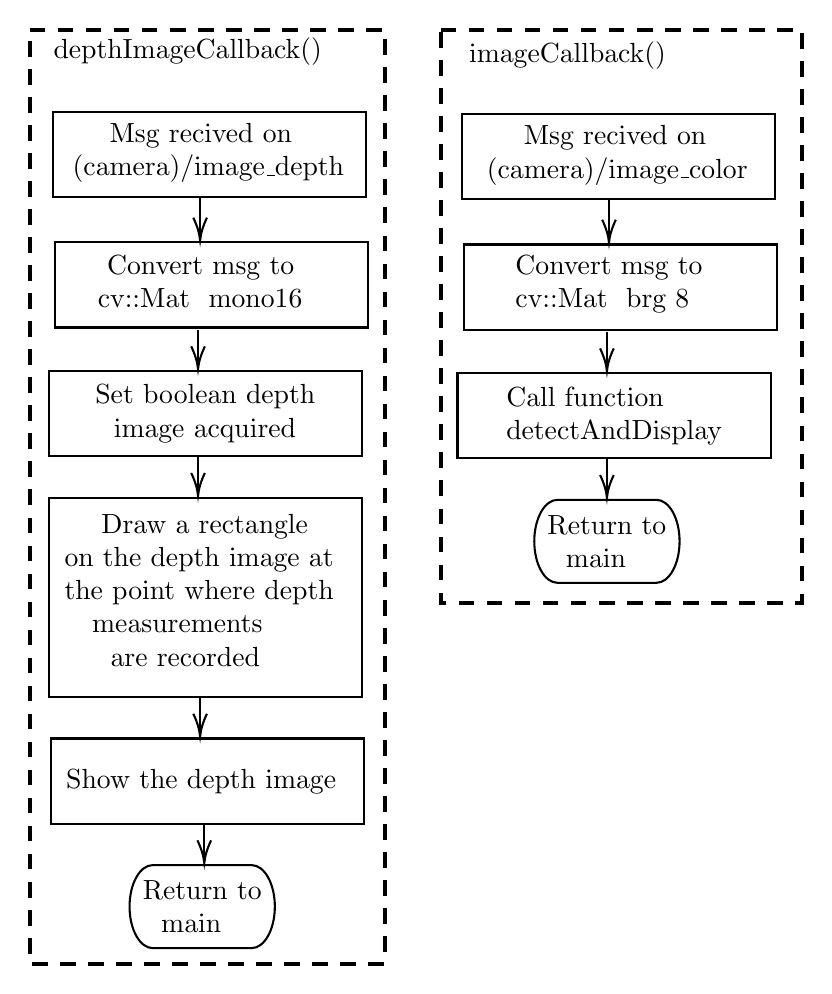
\begin{tikzpicture}[x=0.75pt,y=0.75pt,yscale=-1,xscale=1]
%uncomment if require: \path (0,584.4666595458984); %set diagram left start at 0, and has height of 584.4666595458984

%Flowchart: Process [id:dp02439077301177306] 
\draw   (14,48) -- (165,48) -- (165,89) -- (14,89) -- cycle ;
%Flowchart: Process [id:dp49880928508355205] 
\draw   (15,111) -- (166,111) -- (166,152) -- (15,152) -- cycle ;
%Straight Lines [id:da43939636510498514] 
\draw    (85,89) -- (85,108) ;
\draw [shift={(85,110)}, rotate = 270] [color={rgb, 255:red, 0; green, 0; blue, 0 }  ][line width=0.75]    (10.93,-3.29) .. controls (6.95,-1.4) and (3.31,-0.3) .. (0,0) .. controls (3.31,0.3) and (6.95,1.4) .. (10.93,3.29)   ;

%Flowchart: Process [id:dp17038902478073492] 
\draw   (12,173) -- (163,173) -- (163,214) -- (12,214) -- cycle ;
%Straight Lines [id:da8711474737612683] 
\draw    (84,153) -- (84,170) ;
\draw [shift={(84,172)}, rotate = 270] [color={rgb, 255:red, 0; green, 0; blue, 0 }  ][line width=0.75]    (10.93,-3.29) .. controls (6.95,-1.4) and (3.31,-0.3) .. (0,0) .. controls (3.31,0.3) and (6.95,1.4) .. (10.93,3.29)   ;

%Flowchart: Process [id:dp611891205069492] 
\draw   (12,234) -- (163,234) -- (163,330) -- (12,330) -- cycle ;
%Straight Lines [id:da6189943063787358] 
\draw    (84,214) -- (84,231) ;
\draw [shift={(84,233)}, rotate = 270] [color={rgb, 255:red, 0; green, 0; blue, 0 }  ][line width=0.75]    (10.93,-3.29) .. controls (6.95,-1.4) and (3.31,-0.3) .. (0,0) .. controls (3.31,0.3) and (6.95,1.4) .. (10.93,3.29)   ;

%Flowchart: Process [id:dp8433294446737231] 
\draw   (13,350) -- (164,350) -- (164,391) -- (13,391) -- cycle ;
%Straight Lines [id:da19737824310945895] 
\draw    (85,330) -- (85,347) ;
\draw [shift={(85,349)}, rotate = 270] [color={rgb, 255:red, 0; green, 0; blue, 0 }  ][line width=0.75]    (10.93,-3.29) .. controls (6.95,-1.4) and (3.31,-0.3) .. (0,0) .. controls (3.31,0.3) and (6.95,1.4) .. (10.93,3.29)   ;

%Flowchart: Terminator [id:dp16047304499993764] 
\draw   (62.2,411) -- (109.8,411) .. controls (115.99,411) and (121,419.95) .. (121,431) .. controls (121,442.05) and (115.99,451) .. (109.8,451) -- (62.2,451) .. controls (56.01,451) and (51,442.05) .. (51,431) .. controls (51,419.95) and (56.01,411) .. (62.2,411) -- cycle ;
%Straight Lines [id:da38644975549092275] 
\draw    (87,391) -- (87,408) ;
\draw [shift={(87,410)}, rotate = 270] [color={rgb, 255:red, 0; green, 0; blue, 0 }  ][line width=0.75]    (10.93,-3.29) .. controls (6.95,-1.4) and (3.31,-0.3) .. (0,0) .. controls (3.31,0.3) and (6.95,1.4) .. (10.93,3.29)   ;

%Flowchart: Process [id:dp7304821272489507] 
\draw   (211,49) -- (362,49) -- (362,90) -- (211,90) -- cycle ;
%Flowchart: Process [id:dp6019819619692849] 
\draw   (212,112) -- (363,112) -- (363,153) -- (212,153) -- cycle ;
%Straight Lines [id:da8353367237133162] 
\draw    (282,90) -- (282,109) ;
\draw [shift={(282,111)}, rotate = 270] [color={rgb, 255:red, 0; green, 0; blue, 0 }  ][line width=0.75]    (10.93,-3.29) .. controls (6.95,-1.4) and (3.31,-0.3) .. (0,0) .. controls (3.31,0.3) and (6.95,1.4) .. (10.93,3.29)   ;

%Flowchart: Process [id:dp7252485412567514] 
\draw   (209,174) -- (360,174) -- (360,215) -- (209,215) -- cycle ;
%Straight Lines [id:da24354233707357476] 
\draw    (281,154) -- (281,171) ;
\draw [shift={(281,173)}, rotate = 270] [color={rgb, 255:red, 0; green, 0; blue, 0 }  ][line width=0.75]    (10.93,-3.29) .. controls (6.95,-1.4) and (3.31,-0.3) .. (0,0) .. controls (3.31,0.3) and (6.95,1.4) .. (10.93,3.29)   ;

%Straight Lines [id:da19908387926604076] 
\draw    (281,215) -- (281,232) ;
\draw [shift={(281,234)}, rotate = 270] [color={rgb, 255:red, 0; green, 0; blue, 0 }  ][line width=0.75]    (10.93,-3.29) .. controls (6.95,-1.4) and (3.31,-0.3) .. (0,0) .. controls (3.31,0.3) and (6.95,1.4) .. (10.93,3.29)   ;

%Flowchart: Terminator [id:dp789884812682225] 
\draw   (257.2,235) -- (304.8,235) .. controls (310.99,235) and (316,243.95) .. (316,255) .. controls (316,266.05) and (310.99,275) .. (304.8,275) -- (257.2,275) .. controls (251.01,275) and (246,266.05) .. (246,255) .. controls (246,243.95) and (251.01,235) .. (257.2,235) -- cycle ;
%Shape: Rectangle [id:dp7849222743132149] 
\draw  [dash pattern={on 5.63pt off 4.5pt}][line width=1.5]  (200.92,8.53) -- (374.92,8.53) -- (374.92,284.53) -- (200.92,284.53) -- cycle ;
%Shape: Rectangle [id:dp48715972057195456] 
\draw  [dash pattern={on 5.63pt off 4.5pt}][line width=1.5]  (2.92,8.53) -- (173.92,8.53) -- (173.92,458.53) -- (2.92,458.53) -- cycle ;

% Text Node
\draw (89,68) node  [align=left] { \ \ \ \ Msg recived on \\(camera)/image\_depth};
% Text Node
\draw (85,130) node  [align=left] { \ Convert msg to \\cv::Mat \ mono16};
% Text Node
\draw (87.5,193.5) node  [align=left] { Set boolean depth \\ \ \ image acquired};
% Text Node
\draw (84.5,278.5) node  [align=left] { \ \ \ \ Draw a rectangle\\on the depth image at \\the point where depth\\ \ \ \ measurements\\ \ \ \ \ \ are recorded};
% Text Node
\draw (85.5,377.5) node  [align=left] { Show the depth image\\ };
% Text Node
\draw (86,431) node  [align=left] {Return to \\ \ \ main};
% Text Node
\draw (286,69) node  [align=left] { \ \ \ \ Msg recived on \\(camera)/image\_color};
% Text Node
\draw (282,131) node  [align=left] {Convert msg to \\cv::Mat \ brg 8};
% Text Node
\draw (284.5,194.5) node  [align=left] {Call function \\detectAndDisplay};
% Text Node
\draw (281,255) node  [align=left] { Return to \\ \ \ main};
% Text Node
\draw (79,19) node  [align=left] {depthImageCallback()};
% Text Node
\draw (262,21) node  [align=left] {imageCallback()};


\end{tikzpicture}

